\documentclass[a4paper,UTF8]{article}

\usepackage[margin=1.25in]{geometry}
\usepackage{color}
\usepackage{graphicx}
\usepackage{amssymb}
\usepackage{amsmath}
\usepackage{amsthm}
\usepackage{enumerate}
\usepackage{bm}
\usepackage{hyperref}
\usepackage{epsfig}
\usepackage{color}
\usepackage{mdframed}
\usepackage{lipsum}
\usepackage{mathtools}
\usepackage{algorithm}
\usepackage{algorithmic}
\usepackage{listings}
\usepackage{xcolor}
\usepackage{float}
\usepackage{caption}

\usepackage[utf8]{inputenc}
\usepackage[UTF8]{ctex}

\newmdtheoremenv{thm-box}{myThm}
\newmdtheoremenv{prop-box}{Proposition}
\newmdtheoremenv{def-box}{define}

\setlength{\evensidemargin}{.25in}
\setlength{\textwidth}{6in}
\setlength{\topmargin}{-0.5in}
\setlength{\topmargin}{-0.5in}

\usepackage{indentfirst}
\setlength{\parindent}{2em}

\usepackage{subfigure}
% \setlength{\textheight}{9.5in}
%%%%%%%%%%%%%%%%%%set header and footer here%%%%%%%%%%%%%%%%%%
\usepackage{fancyhdr}
\usepackage{lastpage}
\usepackage{layout}
\footskip = 10pt
\pagestyle{fancy}
\lhead{2020, Spring}
\chead{大数据综合处理实验}
\rhead{实验三}
\cfoot{\thepage}
\renewcommand{\headrulewidth}{1pt}  			%header
\setlength{\skip\footins}{0.5cm}    			
\renewcommand{\footrulewidth}{0pt}  		

\makeatletter 							
\def\headrule{{\if@fancyplain\let\headrulewidth\plainheadrulewidth\fi%
\hrule\@height 1.0pt \@width\headwidth\vskip1pt	
\hrule\@height 0.5pt\@width\headwidth  			
\vskip-2\headrulewidth\vskip-1pt}      			
 \vspace{6mm}}     						
\makeatother

\graphicspath{{img/}}

\lstset{
 columns=fixed,
 basicstyle = \footnotesize,
 breakatwhitespace=false,         % 设置是否当且仅当在空白处自动中断.
 breaklines=true,
 numbers=left,                                        % 在左侧显示行号
 numberstyle=\tiny\color{gray},                       % 设定行号格式
 frame=none,                                          % 不显示背景边框
 backgroundcolor=\color[RGB]{245,245,244},            % 设定背景颜色
 keywordstyle=\color[RGB]{40,40,255},                 % 设定关键字颜色
 numberstyle=\footnotesize\color[RGB]{96,96,96},
 commentstyle=\color[RGB]{0,128,0},                % 设置代码注释的格式
 stringstyle=\rmfamily\slshape\color[RGB]{128,0,0},   % 设置字符串格式
 showstringspaces=false,                              % 不显示字符串中的空格
 language=JAVA,
 extendedchars=true,
 escapeinside=''                                       % 设置语言
}

%%%%%%%%%%%%%%%%%%%%%%%%%%%%%%%%%%%%%%%%%%%%%%
\numberwithin{equation}{section}
\newtheorem{myThm}{myThm}
\newtheorem*{myDef}{Definition}
\newtheorem*{mySol}{Solution}
\newtheorem*{myProof}{Proof}
\newcommand{\indep}{\rotatebox[origin=c]{90}{$\models$}}
\newcommand*\diff{\mathop{}\!\mathrm{d}}

\usepackage{multirow}
\renewcommand\refname{reference}
\author{组长:韩畅,组员:李展烁、王一之、闫旭芃}
\begin{document}
%hello world
%\listoffigures
\captionsetup[figure]{labelfont={bf},labelformat={default},labelsep=period,name={图}}
\title{大数据综合处理实验\\
实验三}
\maketitle

\section{实验规划与设计}
\subsection{任务分配}
{171860551, \text{韩畅:}}\\ \indent
{171860550, \text{王一之:}}\\ \indent
{171860549, \text{闫旭芃:}}\\ \indent
{171840565, \text{李展烁:}}
\subsection{任务要求}
使用 MapReduce 完成两张表的 join 操作
\subsection{设计思路}
实现两张表的join操作,可以利用mapreduce的特性,读入order和product将两张表到map中,将key打包成自定义的数据类型输出,并且按照两表中关联的条件排序依据,将两表满足join条件的数据并携带数据所来源的文件信息,发往同一个reduce task,在reduce中进行数据的串联
\begin{figure}[H]
    \centering

    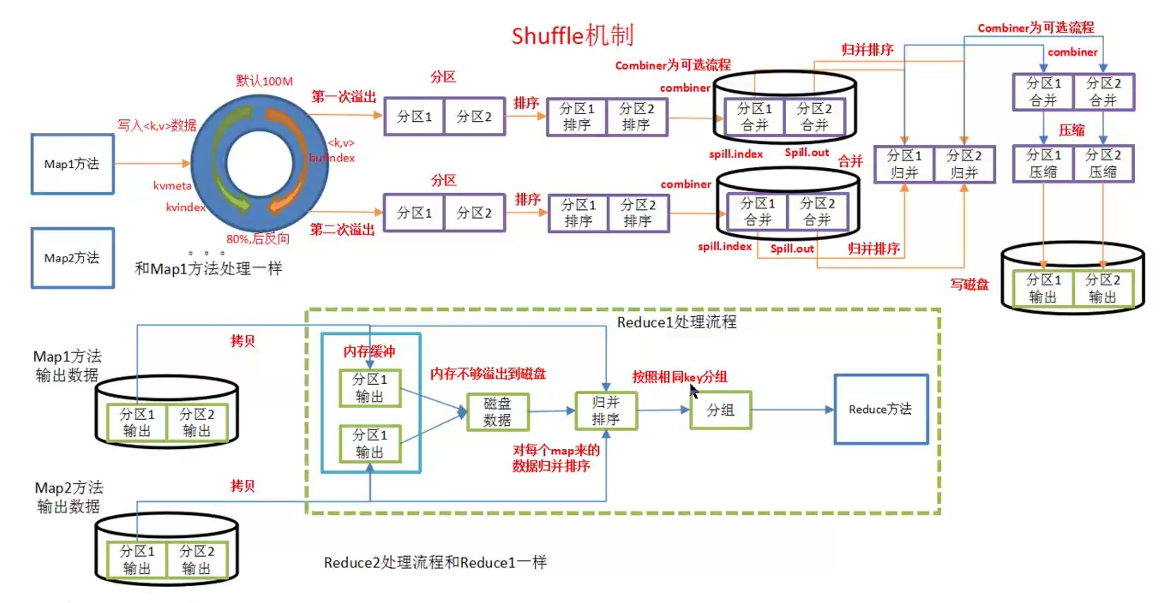
\includegraphics[width = 15cm]{shuffle.png}

    \caption{mapreduce shuffle工作流程图}
\end{figure}
\subsubsection{自定义数据类型}
自定义一个bean存储表中每一种数据:oid,odata,oamount,pid,pname,price
\begin{figure}[H]
    \centering

    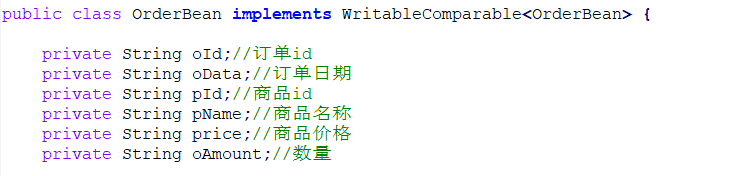
\includegraphics[width = 15cm]{bean1.png}

    \caption{自定义bean}
\end{figure}
实现一些必要的函数,并且实现compareTo(),目的是为了按照pid进行排序分组,每一组然后按照pname排序,因为o表中不存在pname所以,p表中的内容就会被排在o表内容的前面
\begin{figure}[H]
    \centering
    \subfigure[实现compareTo]
    {
        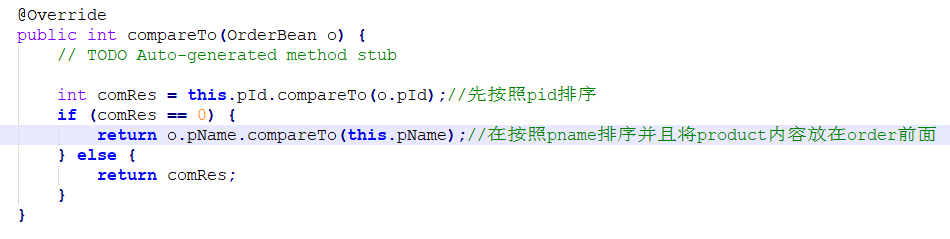
\includegraphics[width = 15cm]{bean2.png}
    }
    \vfill
    \subfigure[部分其他函数(1)]
    {
        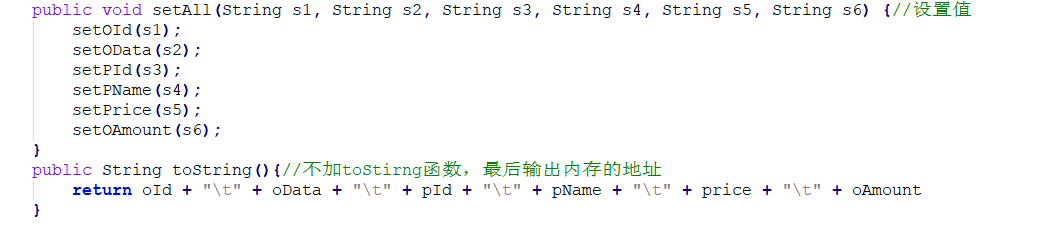
\includegraphics[width = 15cm]{bean3.png}
    }
    \vfill
    \subfigure[部分其他函数(2)]
    {
        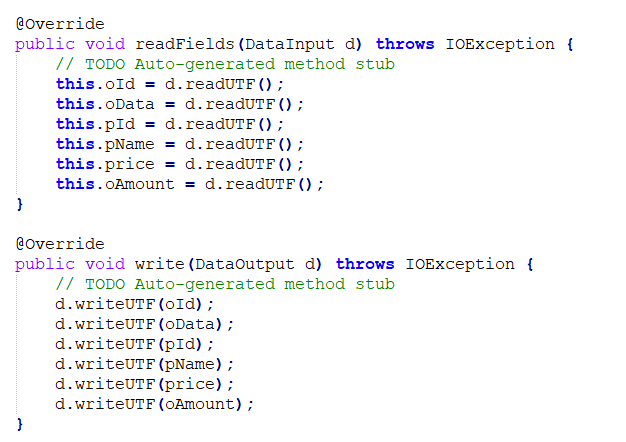
\includegraphics[width = 15cm]{bean4.png}
    }

    \caption{orderbean部分代码实现}
\end{figure}
\subsubsection{主功能Map设计思路}
分辨读入的数据来源于哪个文件,分别给相应的值赋值,不存在的值则赋值为空。输出的key打包成之前自定义的ordebean类型
\begin{figure}[H]
    \centering

    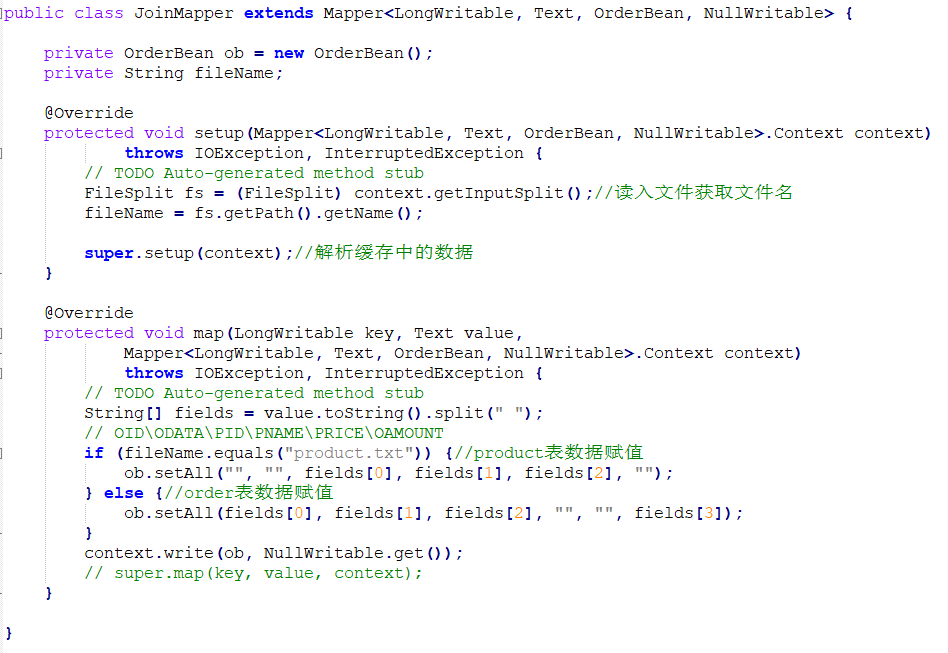
\includegraphics[width = 15cm]{map1.png}

    \caption{mapper部分实现}
\end{figure}
\subsubsection{重写Partitioner}
对map发出的数据进行分区,根据pid进行分区
\begin{figure}[H]
    \centering

    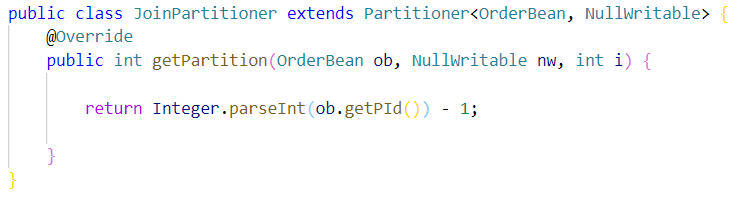
\includegraphics[width = 15cm]{part1.png}

    \caption{mapper部分实现}
\end{figure}
\subsubsection{排序}
排序会根据key排序,由于key是自定义数据类型orderbean,所以在orderbean中需要自定义排序方法(见上)compareTo函数
首先按照pid排序,然后按照pname排序。由于product中pid 是唯一的,所以相同的pid中只会有一个pname,并且会被排序到最前面,形成特定的结构
\begin{figure}[H]
    \centering
    \subfigure[按照pid进行排序]
    {
        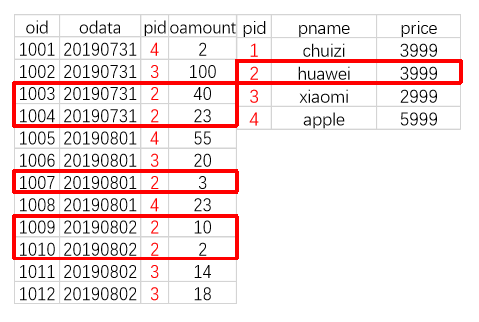
\includegraphics[width = 15cm]{ord1.png}
    }
    \vfill
    \subfigure[排序结果示例]
    {
        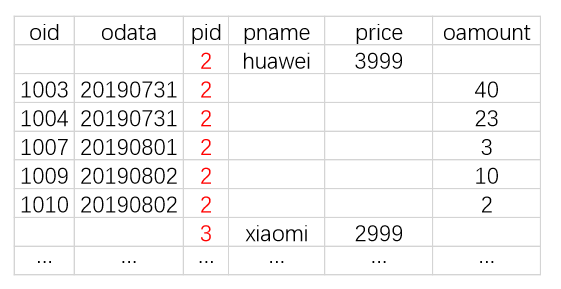
\includegraphics[width = 15cm]{ord2.png}
    }
    \caption{排序示例}
\end{figure}
\subsubsection{自定义分组}
一个reduce任务,默认只会接收到一个key的数据,所以我们要把相同pid的数据分到一个组里面处理
\begin{figure}[H]
    \centering

    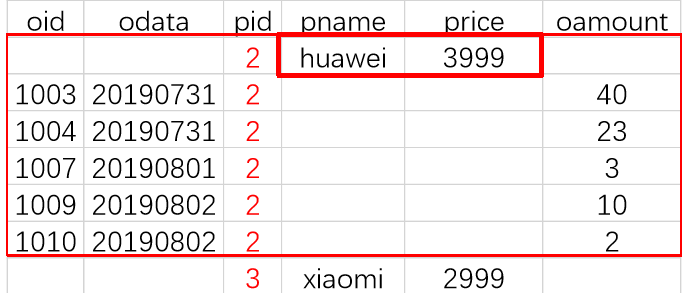
\includegraphics[width = 15cm]{comp1.png}

    \caption{自定义分组示例}
\end{figure}
\begin{figure}[H]
    \centering

    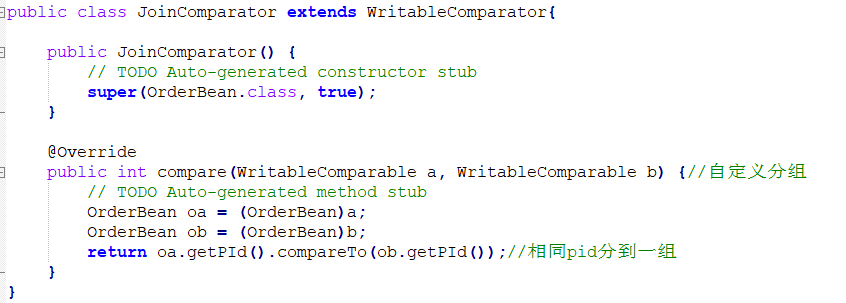
\includegraphics[width = 15cm]{comp2.png}

    \caption{重写Comparator}
\end{figure}
\subsubsection{主功能Reduce设计思路}
TODO:   主功能Reduce设计思路


\subsubsection{Key-Value类型协调}
value设为空NullWritable,自定义key数据类型OrderBean,将数据全部封装到这里面,方便后续排序,分区,分组
\subsection{代码演示}
\subsubsection{Map阶段代码演示}
已经包含在设计思路图片中

\subsubsection{Reduce阶段代码演示}

\section{实验结果展示}
\subsection{结果文件截图}

\subsection{结果文件在HDFS上的路径}
/user/2020st18/output2/
\subsection{所有命令}
jar包执行命令:hadoop jar /home/2020st18/HiveMyJoin.jar MyJoin.JoinDriver /data/exercise\_3 output2 

hive建表命令:create table orders(id int,order\_date string,pid string,name string,price int,num int) row format delimited fields terminated by '\t' location '/user/2020st18/output2/';
\subsection{hive 输出结果文件的部分截图}
\begin{figure}[H]
	\centering
	\subfigure[orders表开头]
	{
		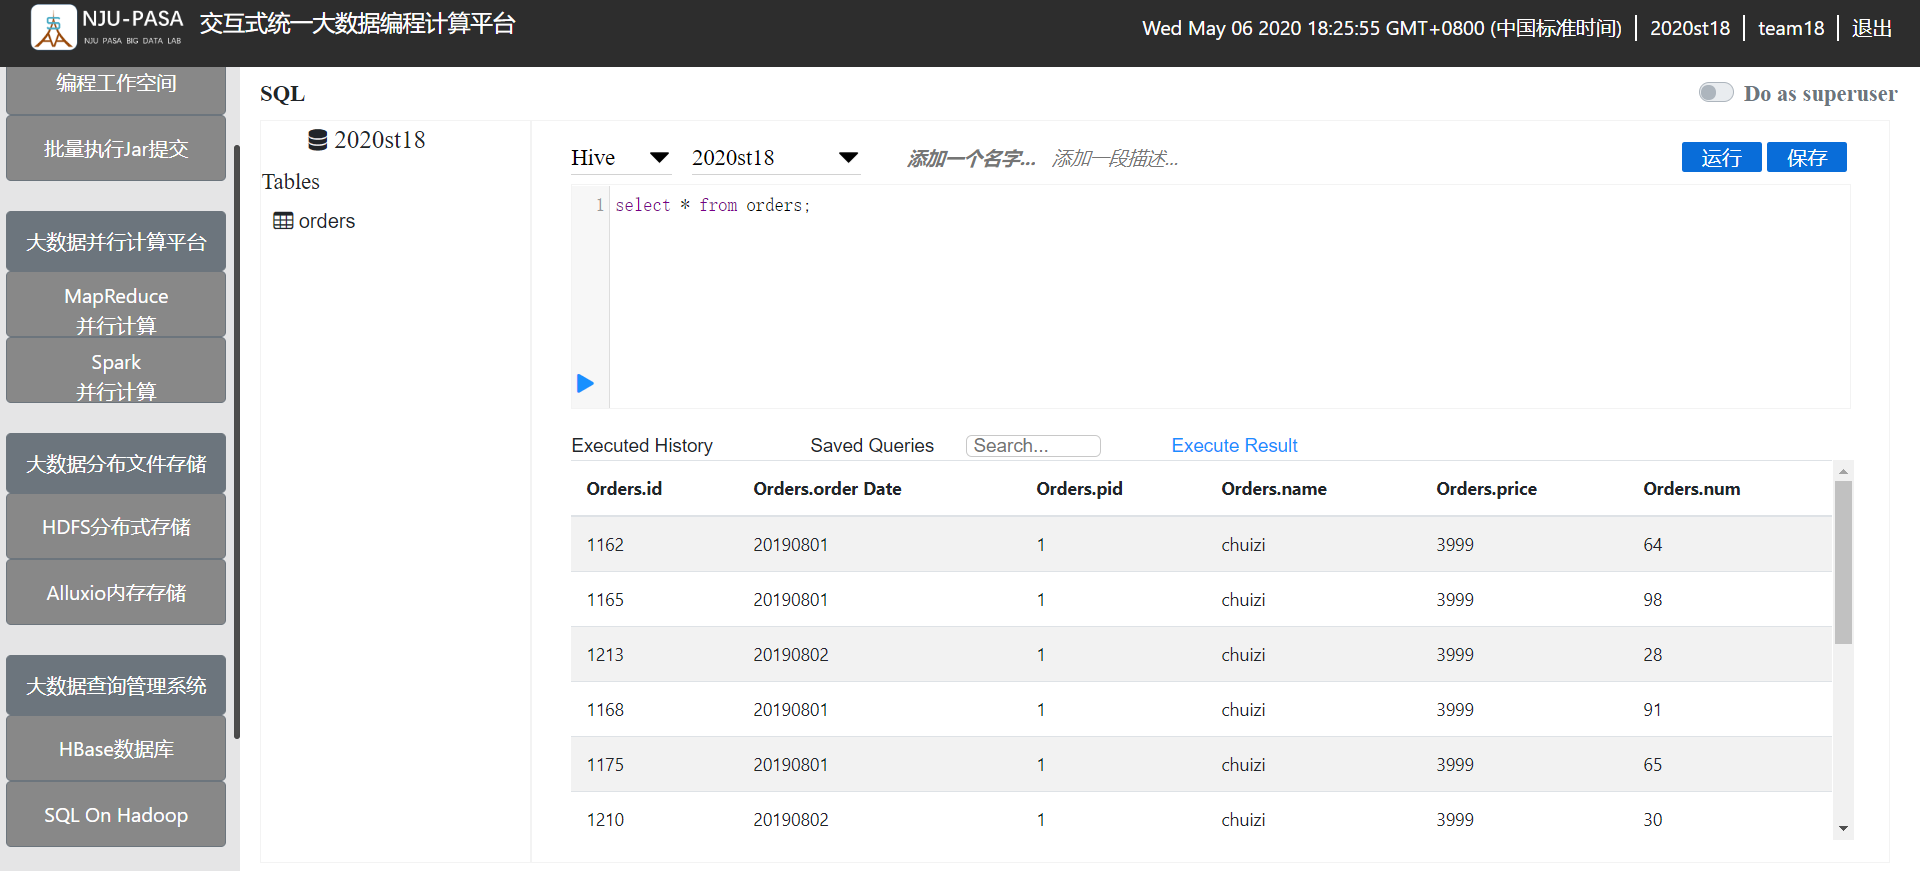
\includegraphics[width = 15cm]{hive1.PNG}
	}
	\vfill
	\subfigure[orders表结尾]
	{
		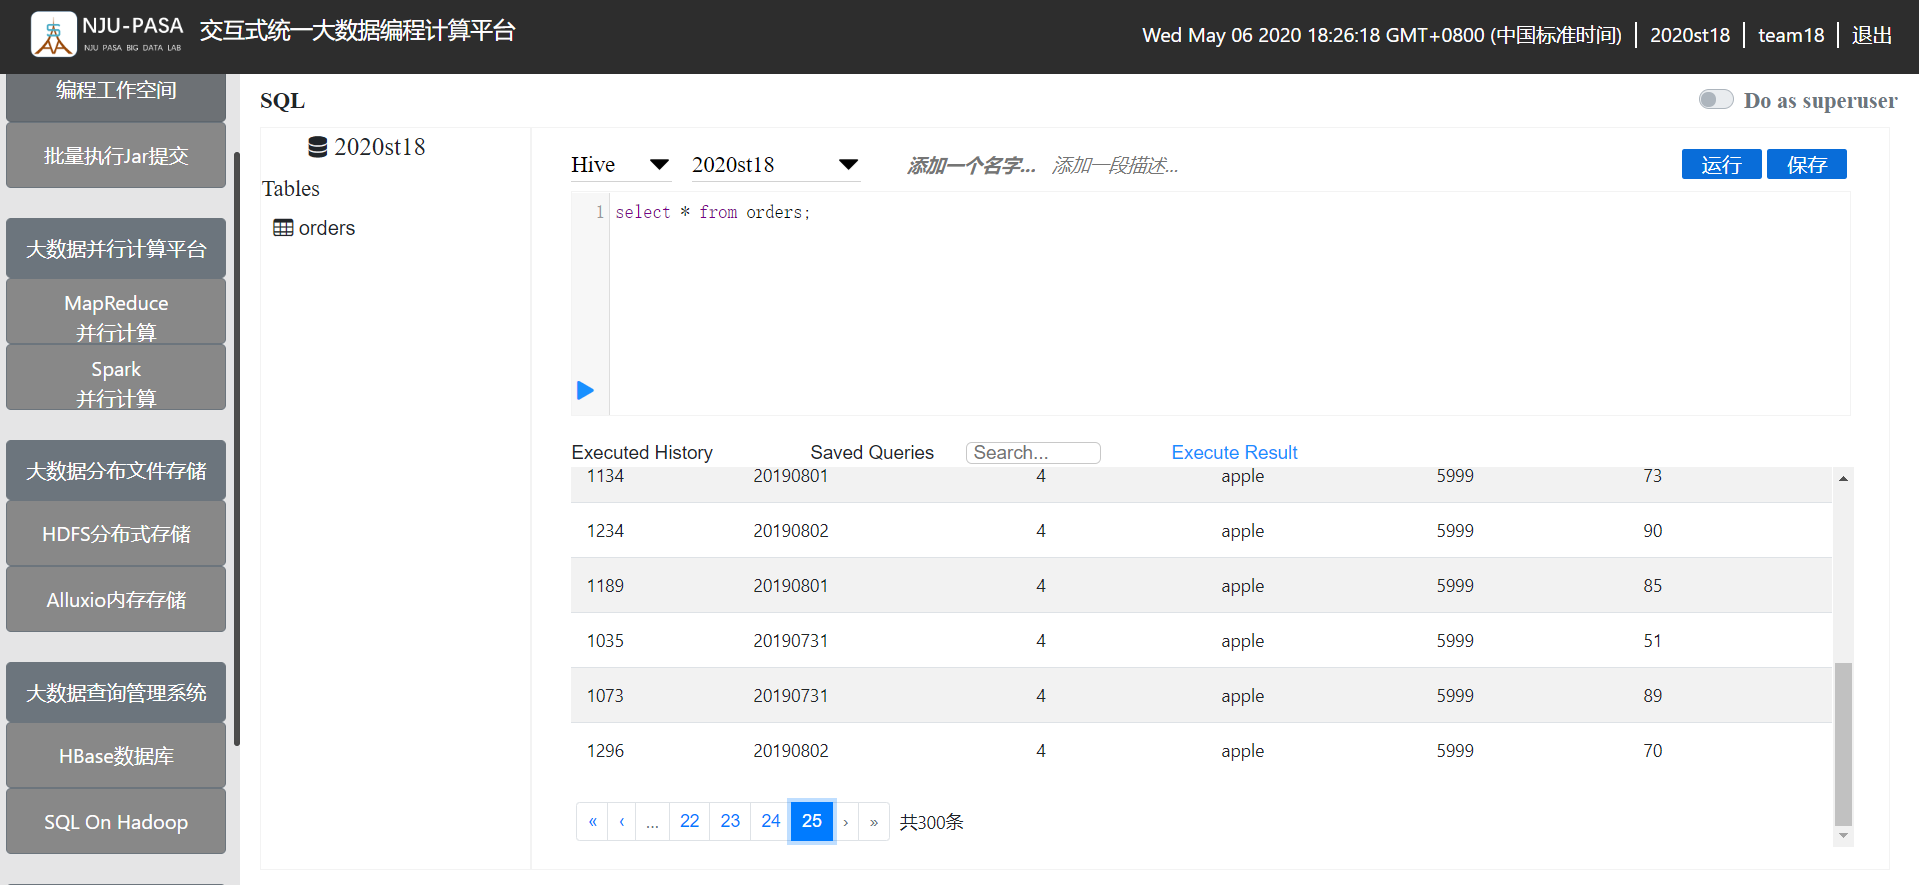
\includegraphics[width = 15cm]{hive2.PNG}
	}
	
	\caption{Hive执行结果}
\end{figure}
\subsection{Web UI 报告内容展示}
\begin{figure}[H]
	\centering
	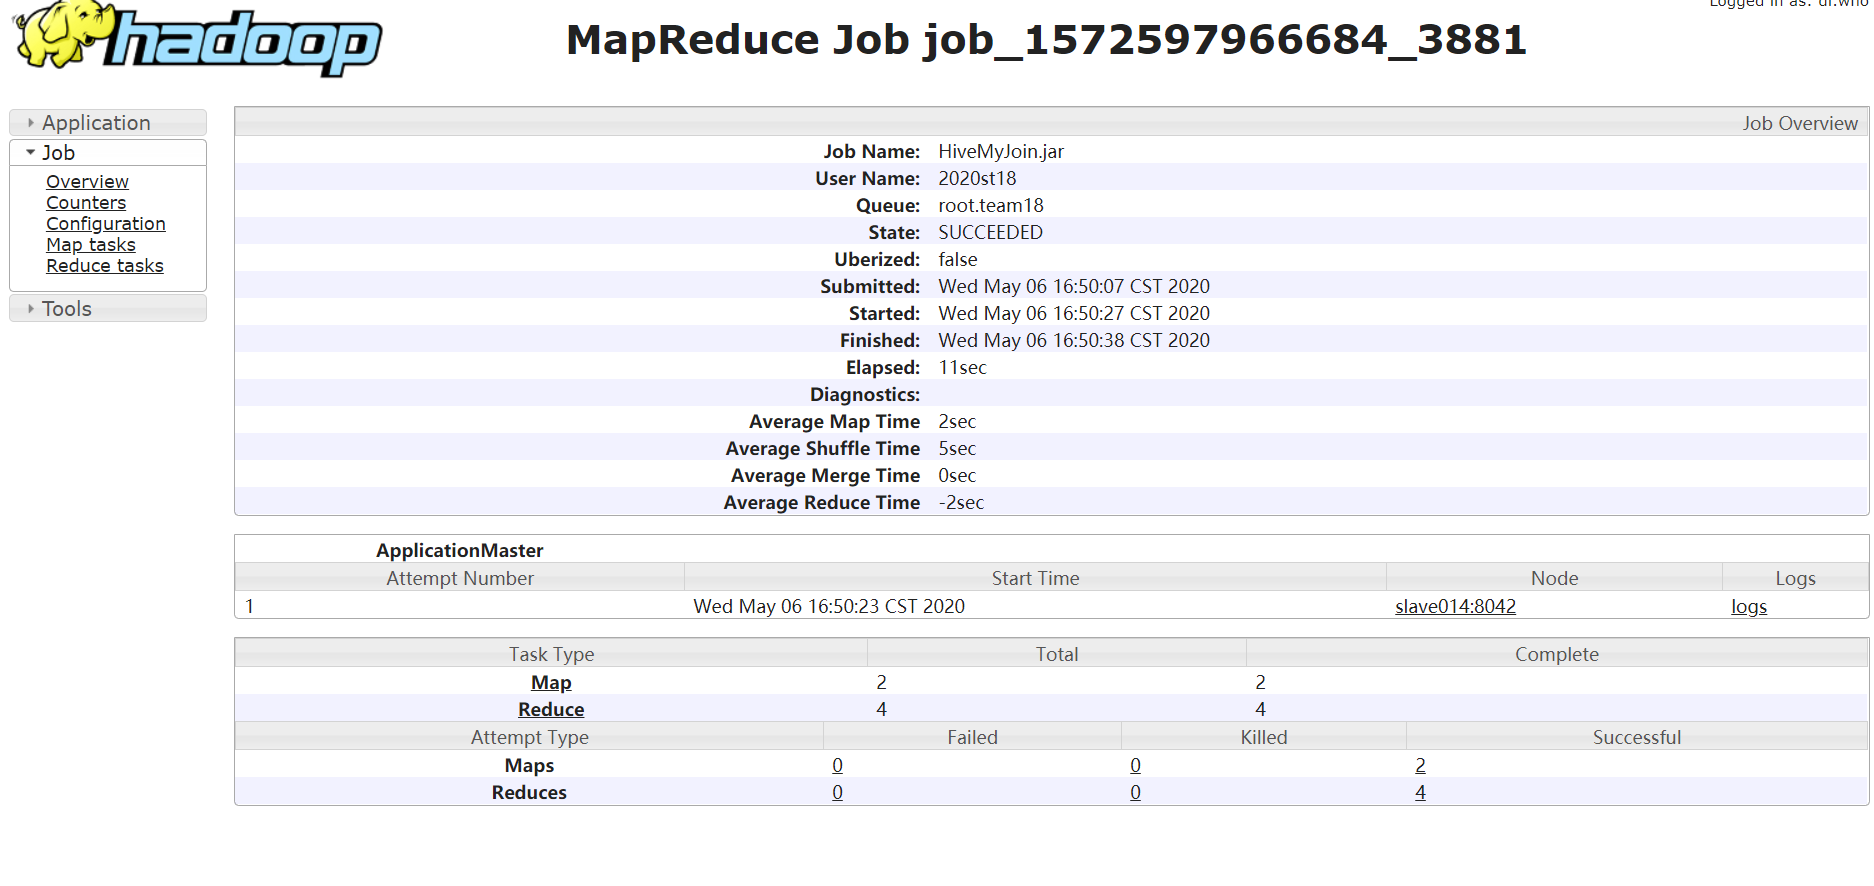
\includegraphics[width = 15cm]{job.PNG}
	\caption{WebUI执行报告}
\end{figure}
\section{实验经验总结与改进方向}



% 下面是插入多个图片的示例代码

% \begin{figure}[htbp]
%     \centering

%     \subfigure[lenna-origin-rgb]
%     {
%     \label{fig1a}
%     \includegraphics[height = 4cm]{lenna.png}
%     }
%     \hspace{1cm} % 设置图间距离
%     \subfigure[lenna-origin-gray]
%     {
%     \label{fig1b}
%     \includegraphics[height = 4cm]{img/lennaGray.png}
%     }

%     \vfill % 换行
%     \subfigure[lenna-matlab-fil0]{
%         \label{fig1c}
%         \includegraphics[height = 4cm]{img/lennaGrayFilCtrGrp.png}
%     }
%     \hspace{1cm}
%     \subfigure[lenna-my-fil0]{
%         \label{fig1d}
%         \includegraphics[height = 4cm]{img/lennaGrayFil0My.png}
%     }
%       %设置配图文字
%     \caption{We notice that the image generating by matlab's filter has black edge all around the output image, while our own filter only make the black edge at the upper left corner due to different 0-padding rules.}
%     \label{fig1}
% \end{figure}



\bibliographystyle{plain}
\bibliography{ref}

\end{document}
